\documentclass[NET,english,beameralt]{tumbeamer}
\usepackage[options]{minted}
\usepackage[options]{hyperref}
% Configure author, title, etc. here:
\documentclass[NET,english,beameralt]{tumbeamer}
\usepackage[options]{minted}
\usepackage[options]{hyperref}
\documentclass[NET,english,beameralt]{tumbeamer}
\usepackage[options]{minted}
\usepackage[options]{hyperref}
\documentclass[NET,english,beameralt]{tumbeamer}
\usepackage[options]{minted}
\usepackage[options]{hyperref}
\input{include/slides}
\beamerdefaultoverlayspecification{<+->}

\begin{document}

\begin{frame}{Agenda}
    \begin{itemize}[<.->]
        \item Starlink 101
        \item trying to understand routing decisions
        \item visualize visible satellites
        \item exploring the GRPC api
    \end{itemize}
\end{frame}

\begin{frame}{Starlink 101}
\begin{figure}
    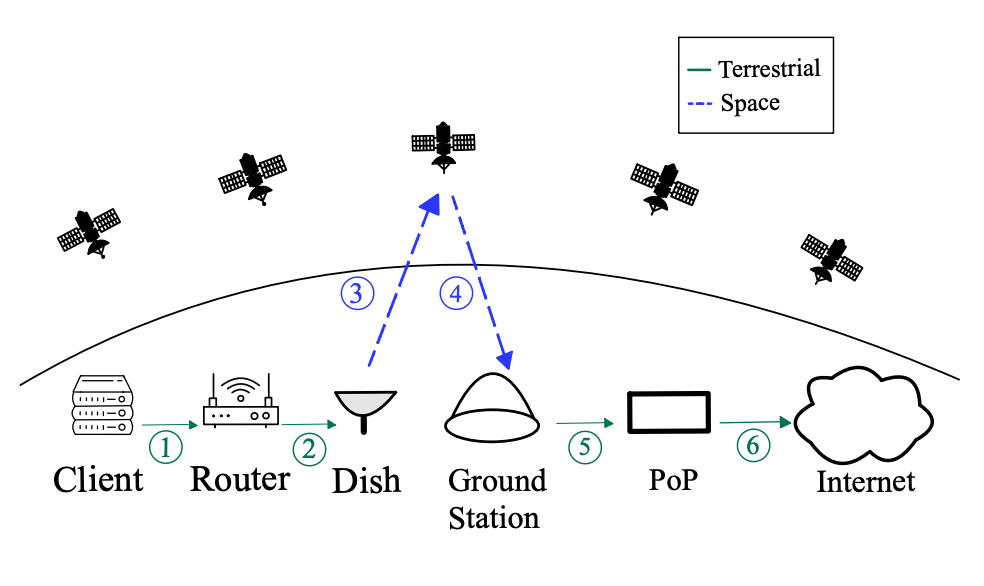
\includegraphics[width=0.75\textwidth]{pics/starlink-101.png}
    \caption[short]{Basic Starlink working (ignoring ISL), from \cite{izhikevich2023democratizing}}
\end{figure}
\end{frame}

\begin{frame}{Understanding routing decisions}
\begin{itemize}
    \item got ip address blocks from major cloud providers (aws,azure,oracle), as we know their position \footnote[]{the fact we know the position doesn't really mean a traceroute to a certain address is really a traceroute to that geographic area}
    \item chose 5 geographically sparse targets around the globe (for aws: ap-northeast-2, us-east-1, ap-south-1, sa-east-1, me-south-1 )
    \item tracerouted the targets over several days 
\end{itemize}
\end{frame}

\begin{frame}{Understanding routing decisions}
\begin{figure}
    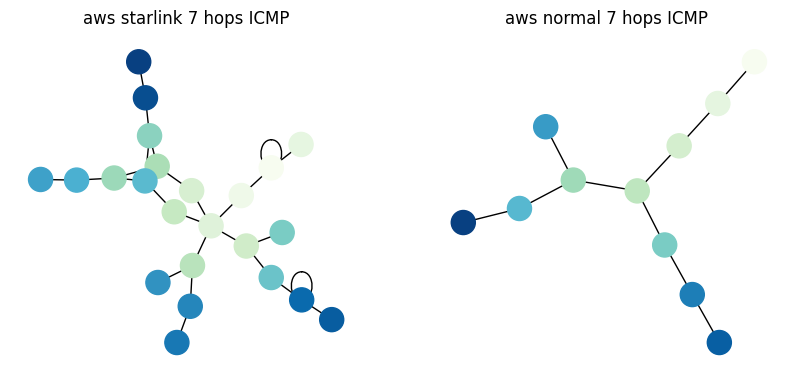
\includegraphics[width=0.75\textwidth]{pics/aws_7_icmp.png}
    \caption[short]{First 7 hops of traceroutes to 5 AWS datacenters using ICMP}
\end{figure}
\end{frame}

\begin{frame}{Understanding routing decisions}
\begin{figure}
    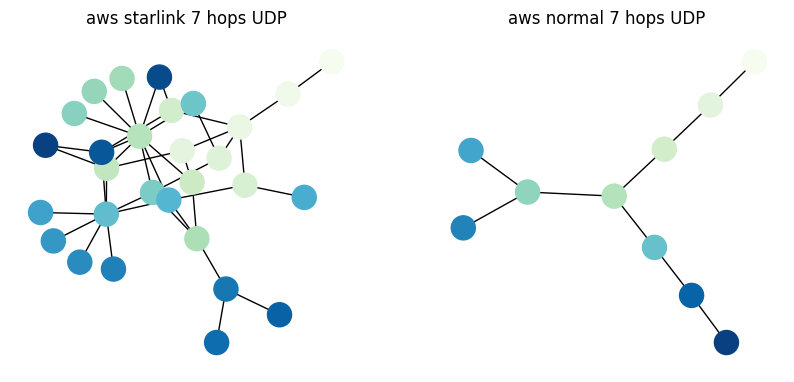
\includegraphics[width=0.75\textwidth]{pics/aws_7_udp.png}
    \caption[short]{First 7 hops of traceroutes to 5 AWS datacenters using UDP}
\end{figure}
\end{frame}

\begin{frame}{Understanding routing decisions}
\begin{figure}
    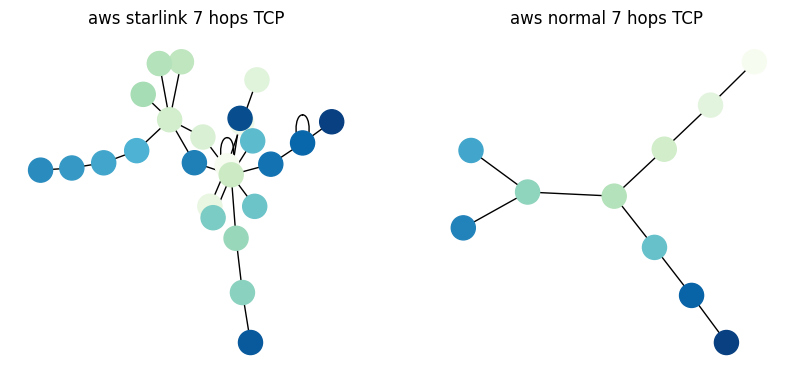
\includegraphics[width=0.75\textwidth]{pics/aws_7_tcp.png}
    \caption[short]{First 7 hops of traceroutes to 5 AWS datacenters using TCP}
\end{figure}
\end{frame}

\begin{frame}{measuring RTT changes when applying stress iperf}
\begin{figure}
    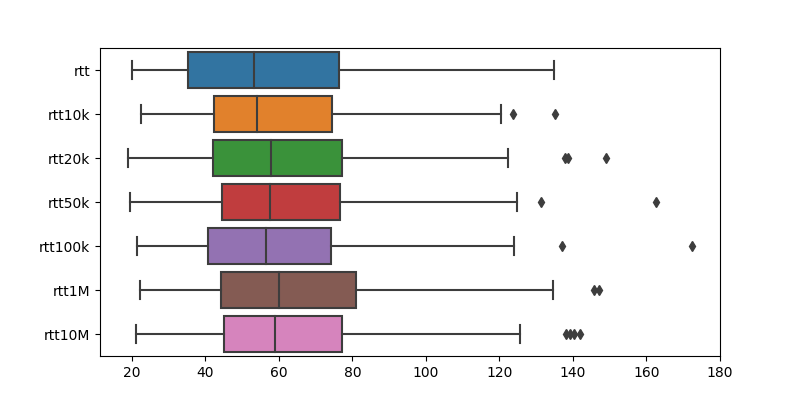
\includegraphics[width=1\textwidth]{pics/rtt-iperf-stress.png}
    \caption[short]{measuring RTT changes when applying stress iperf}
\end{figure}
\end{frame}

\begin{frame}{Visualize visible satellites}
\begin{itemize}
    \item from \href{celestrak.org}{celestrak.org} we can download a list of Starlink's satellites TLEs
    \item A two-line element set (TLE) is a data format encoding a list of orbital elements of an Earth-orbiting object for a given point in time, the epoch. Using a suitable prediction formula, the state (position and velocity) at any point in the past or future can be estimated to some accuracy. (from wikipedia.org)
\end{itemize}
\end{frame}

\begin{frame}[fragile]{\texttt{common.calculate\_visible\_satellites}}
\begin{minted}[fontsize=\small]{python3}
def calculate_visible_satellites(...):
    # ...
    satellites = load.tle_file(stations_url)
    observer = Topos(observer_latitude, observer_longitude, observer_elevation)
    t = load.timescale().now()

    # Calculate satellite positions
    positions = [(sat, (sat - observer).at(t)) for sat in satellites]
    
    # Filter visible satellites
    visible_satellites = []
    for sat, position in positions:
        alt, az, distance = position.altaz()
        # Satellite is above the horizon
        if alt.degrees > 0 and distance.km < distance_km:
            visible_satellites.append((sat, alt, az))

    return visible_satellites
\end{minted}
\end{frame}

\begin{frame}{count of visible satellites across time}
\begin{figure}
    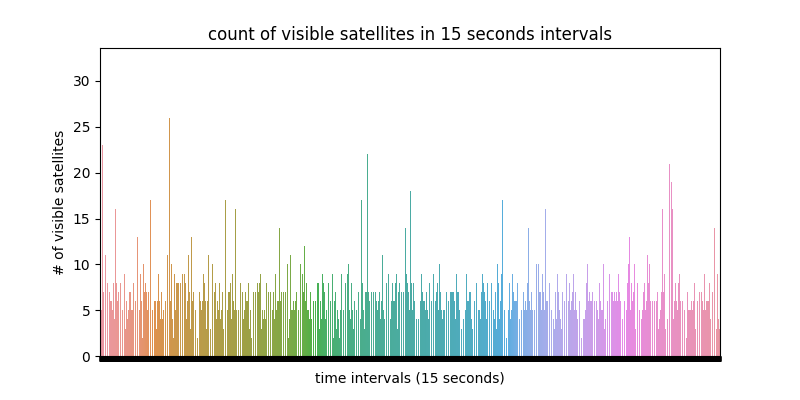
\includegraphics[width=1\textwidth]{pics/count_visible_satellites.png}
    \caption[short]{count of visible satellites across time}
\end{figure}
\end{frame}

\begin{frame}{visualizing patterns in visible satellites}
\begin{figure}
    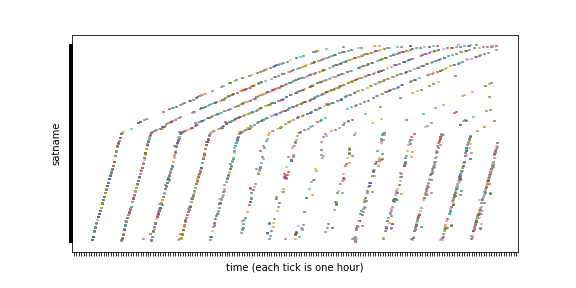
\includegraphics[width=1\textwidth]{pics/visualizing-how-long-satellites-are-visible-for.png}
    \caption[short]{visualizing patterns in visible satellites}
\end{figure}
\end{frame}

\begin{frame}{the gRPC api}
\begin{itemize}
    \item the dish exposes a gRPC api with server reflection, "runtime construction of requests without having stub information precompiled into the client." \footnote{\href{https://github.com/grpc/grpc/blob/master/doc/server-reflection.md}{https://github.com/grpc/grpc/blob/master/doc/server-reflection.md}}
    \item 55 "methods" are available, most of them don't work, we have 2 categories of errors: \texttt{Uninmplemented}, \texttt{PermissionDenied} and a couple of some other specific errors 
    \item working methods: \texttt{reboot}, \texttt{get\_status}, \texttt{start\_dish\_self\_test}, \texttt{get\_history}, \texttt{get\_device\_info}, \texttt{dish\_power\_save}, \texttt{dish\_get\_config}, \texttt{get\_obstruction\_map}
    \item to see all methods: \href{https://hedgedoc.net.in.tum.de/N7nACD1OSk2x2e7biPHJTA}{https://hedgedoc.net.in.tum.de/N7nACD1OSk2x2e7biPHJTA}
\end{itemize}
\end{frame}

\begin{frame}{next actions}
\begin{itemize}
    \item investigate satellite handovers following the method described in \cite{izhikevich2023democratizing} (we have a script working)
    \item try to correlate satellite handovers with sudden drops in bandwidth
    \item sneak peak: \href{https://youtu.be/PjfMPr20suw}{https://youtu.be/PjfMPr20suw}
\end{itemize}
\end{frame}

\section{Bibliography}
\begin{frame}[allowframebreaks]
    \bibliographystyle{abbrv}
    \setbeamertemplate{bibliography item}[text]
    \footnotesize
    \bibliography{lit}
\end{frame}

\end{document}

\beamerdefaultoverlayspecification{<+->}

\begin{document}

\begin{frame}{Agenda}
    \begin{itemize}[<.->]
        \item Starlink 101
        \item trying to understand routing decisions
        \item visualize visible satellites
        \item exploring the GRPC api
    \end{itemize}
\end{frame}

\begin{frame}{Starlink 101}
\begin{figure}
    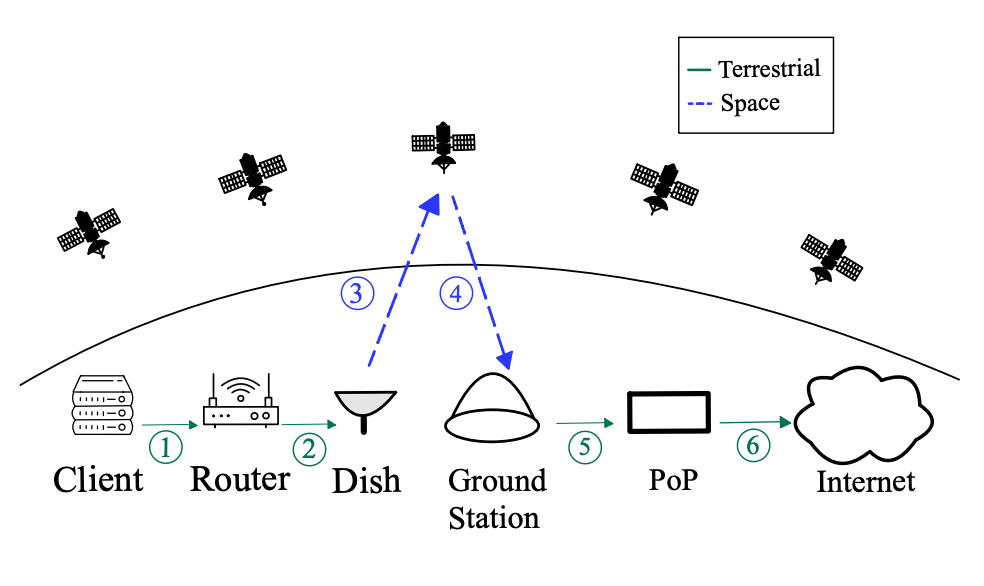
\includegraphics[width=0.75\textwidth]{pics/starlink-101.png}
    \caption[short]{Basic Starlink working (ignoring ISL), from \cite{izhikevich2023democratizing}}
\end{figure}
\end{frame}

\begin{frame}{Understanding routing decisions}
\begin{itemize}
    \item got ip address blocks from major cloud providers (aws,azure,oracle), as we know their position \footnote[]{the fact we know the position doesn't really mean a traceroute to a certain address is really a traceroute to that geographic area}
    \item chose 5 geographically sparse targets around the globe (for aws: ap-northeast-2, us-east-1, ap-south-1, sa-east-1, me-south-1 )
    \item tracerouted the targets over several days 
\end{itemize}
\end{frame}

\begin{frame}{Understanding routing decisions}
\begin{figure}
    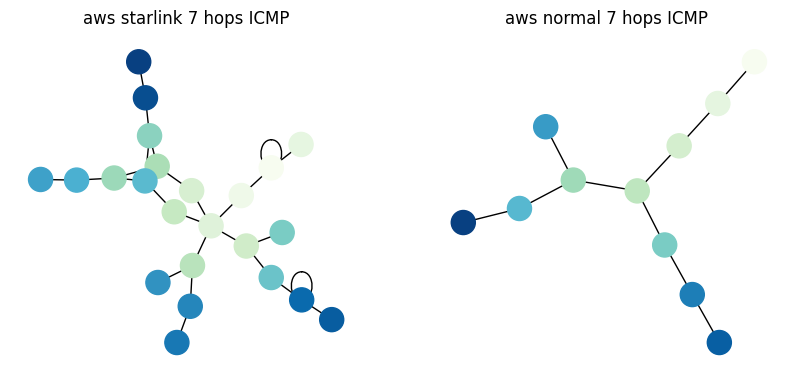
\includegraphics[width=0.75\textwidth]{pics/aws_7_icmp.png}
    \caption[short]{First 7 hops of traceroutes to 5 AWS datacenters using ICMP}
\end{figure}
\end{frame}

\begin{frame}{Understanding routing decisions}
\begin{figure}
    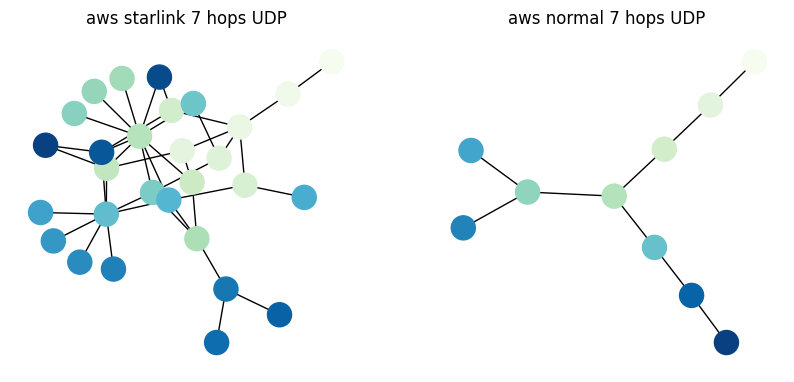
\includegraphics[width=0.75\textwidth]{pics/aws_7_udp.png}
    \caption[short]{First 7 hops of traceroutes to 5 AWS datacenters using UDP}
\end{figure}
\end{frame}

\begin{frame}{Understanding routing decisions}
\begin{figure}
    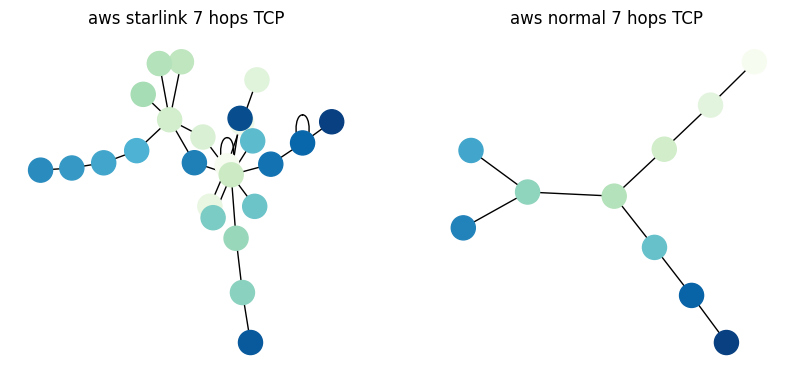
\includegraphics[width=0.75\textwidth]{pics/aws_7_tcp.png}
    \caption[short]{First 7 hops of traceroutes to 5 AWS datacenters using TCP}
\end{figure}
\end{frame}

\begin{frame}{measuring RTT changes when applying stress iperf}
\begin{figure}
    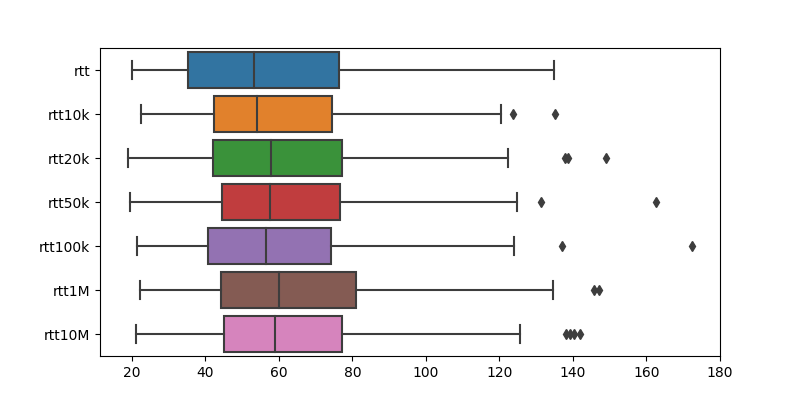
\includegraphics[width=1\textwidth]{pics/rtt-iperf-stress.png}
    \caption[short]{measuring RTT changes when applying stress iperf}
\end{figure}
\end{frame}

\begin{frame}{Visualize visible satellites}
\begin{itemize}
    \item from \href{celestrak.org}{celestrak.org} we can download a list of Starlink's satellites TLEs
    \item A two-line element set (TLE) is a data format encoding a list of orbital elements of an Earth-orbiting object for a given point in time, the epoch. Using a suitable prediction formula, the state (position and velocity) at any point in the past or future can be estimated to some accuracy. (from wikipedia.org)
\end{itemize}
\end{frame}

\begin{frame}[fragile]{\texttt{common.calculate\_visible\_satellites}}
\begin{minted}[fontsize=\small]{python3}
def calculate_visible_satellites(...):
    # ...
    satellites = load.tle_file(stations_url)
    observer = Topos(observer_latitude, observer_longitude, observer_elevation)
    t = load.timescale().now()

    # Calculate satellite positions
    positions = [(sat, (sat - observer).at(t)) for sat in satellites]
    
    # Filter visible satellites
    visible_satellites = []
    for sat, position in positions:
        alt, az, distance = position.altaz()
        # Satellite is above the horizon
        if alt.degrees > 0 and distance.km < distance_km:
            visible_satellites.append((sat, alt, az))

    return visible_satellites
\end{minted}
\end{frame}

\begin{frame}{count of visible satellites across time}
\begin{figure}
    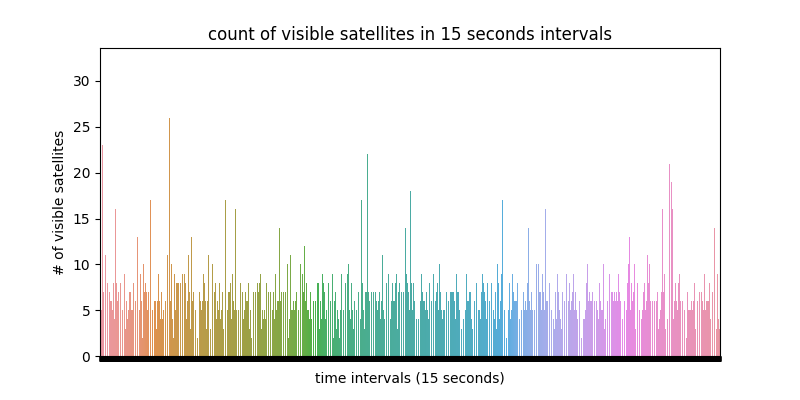
\includegraphics[width=1\textwidth]{pics/count_visible_satellites.png}
    \caption[short]{count of visible satellites across time}
\end{figure}
\end{frame}

\begin{frame}{visualizing patterns in visible satellites}
\begin{figure}
    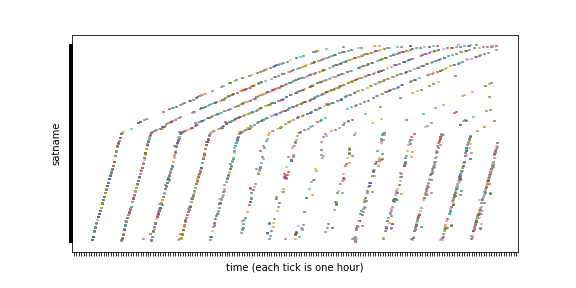
\includegraphics[width=1\textwidth]{pics/visualizing-how-long-satellites-are-visible-for.png}
    \caption[short]{visualizing patterns in visible satellites}
\end{figure}
\end{frame}

\begin{frame}{the gRPC api}
\begin{itemize}
    \item the dish exposes a gRPC api with server reflection, "runtime construction of requests without having stub information precompiled into the client." \footnote{\href{https://github.com/grpc/grpc/blob/master/doc/server-reflection.md}{https://github.com/grpc/grpc/blob/master/doc/server-reflection.md}}
    \item 55 "methods" are available, most of them don't work, we have 2 categories of errors: \texttt{Uninmplemented}, \texttt{PermissionDenied} and a couple of some other specific errors 
    \item working methods: \texttt{reboot}, \texttt{get\_status}, \texttt{start\_dish\_self\_test}, \texttt{get\_history}, \texttt{get\_device\_info}, \texttt{dish\_power\_save}, \texttt{dish\_get\_config}, \texttt{get\_obstruction\_map}
    \item to see all methods: \href{https://hedgedoc.net.in.tum.de/N7nACD1OSk2x2e7biPHJTA}{https://hedgedoc.net.in.tum.de/N7nACD1OSk2x2e7biPHJTA}
\end{itemize}
\end{frame}

\begin{frame}{next actions}
\begin{itemize}
    \item investigate satellite handovers following the method described in \cite{izhikevich2023democratizing} (we have a script working)
    \item try to correlate satellite handovers with sudden drops in bandwidth
    \item sneak peak: \href{https://youtu.be/PjfMPr20suw}{https://youtu.be/PjfMPr20suw}
\end{itemize}
\end{frame}

\section{Bibliography}
\begin{frame}[allowframebreaks]
    \bibliographystyle{abbrv}
    \setbeamertemplate{bibliography item}[text]
    \footnotesize
    \bibliography{lit}
\end{frame}

\end{document}

\beamerdefaultoverlayspecification{<+->}

\begin{document}

\begin{frame}{Agenda}
    \begin{itemize}[<.->]
        \item Starlink 101
        \item trying to understand routing decisions
        \item visualize visible satellites
        \item exploring the GRPC api
    \end{itemize}
\end{frame}

\begin{frame}{Starlink 101}
\begin{figure}
    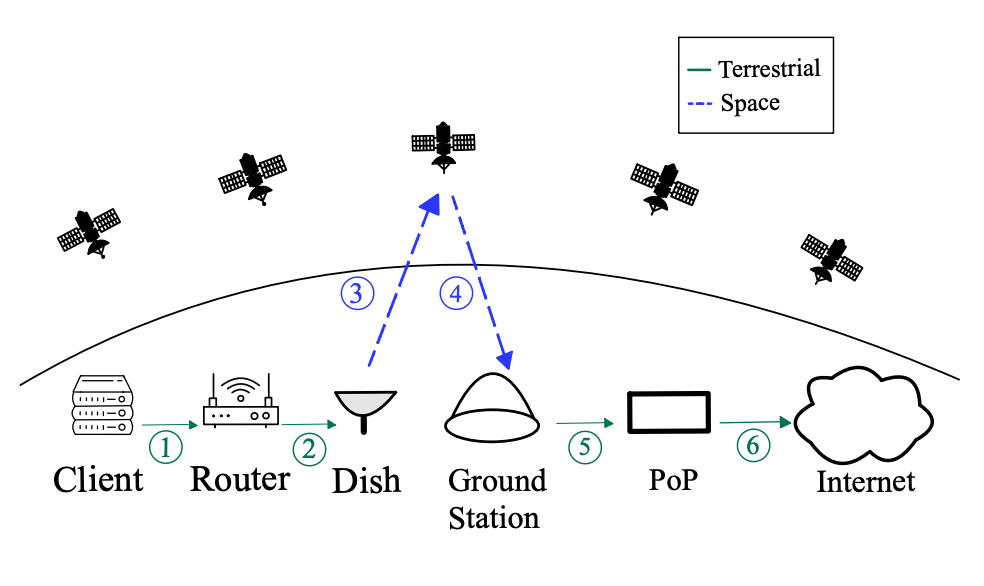
\includegraphics[width=0.75\textwidth]{pics/starlink-101.png}
    \caption[short]{Basic Starlink working (ignoring ISL), from \cite{izhikevich2023democratizing}}
\end{figure}
\end{frame}

\begin{frame}{Understanding routing decisions}
\begin{itemize}
    \item got ip address blocks from major cloud providers (aws,azure,oracle), as we know their position \footnote[]{the fact we know the position doesn't really mean a traceroute to a certain address is really a traceroute to that geographic area}
    \item chose 5 geographically sparse targets around the globe (for aws: ap-northeast-2, us-east-1, ap-south-1, sa-east-1, me-south-1 )
    \item tracerouted the targets over several days 
\end{itemize}
\end{frame}

\begin{frame}{Understanding routing decisions}
\begin{figure}
    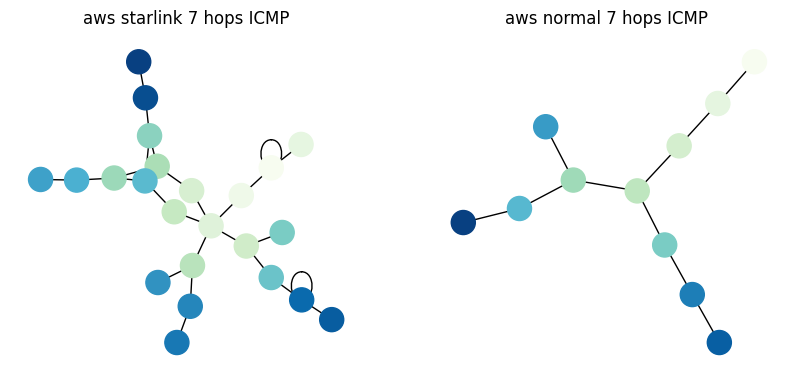
\includegraphics[width=0.75\textwidth]{pics/aws_7_icmp.png}
    \caption[short]{First 7 hops of traceroutes to 5 AWS datacenters using ICMP}
\end{figure}
\end{frame}

\begin{frame}{Understanding routing decisions}
\begin{figure}
    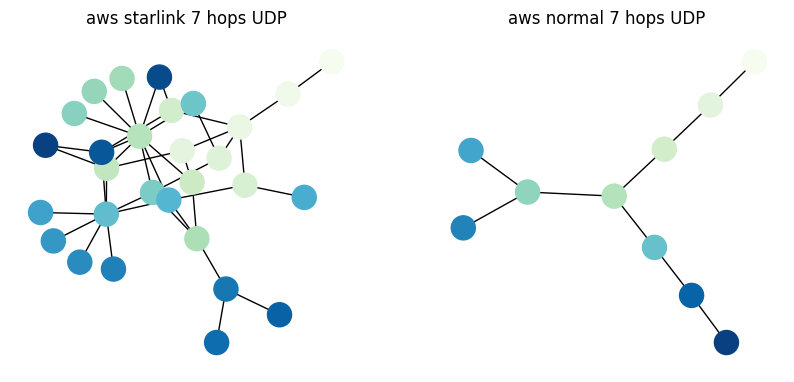
\includegraphics[width=0.75\textwidth]{pics/aws_7_udp.png}
    \caption[short]{First 7 hops of traceroutes to 5 AWS datacenters using UDP}
\end{figure}
\end{frame}

\begin{frame}{Understanding routing decisions}
\begin{figure}
    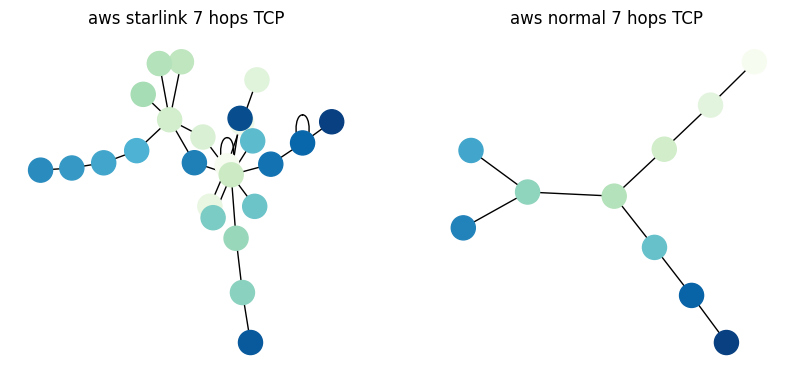
\includegraphics[width=0.75\textwidth]{pics/aws_7_tcp.png}
    \caption[short]{First 7 hops of traceroutes to 5 AWS datacenters using TCP}
\end{figure}
\end{frame}

\begin{frame}{measuring RTT changes when applying stress iperf}
\begin{figure}
    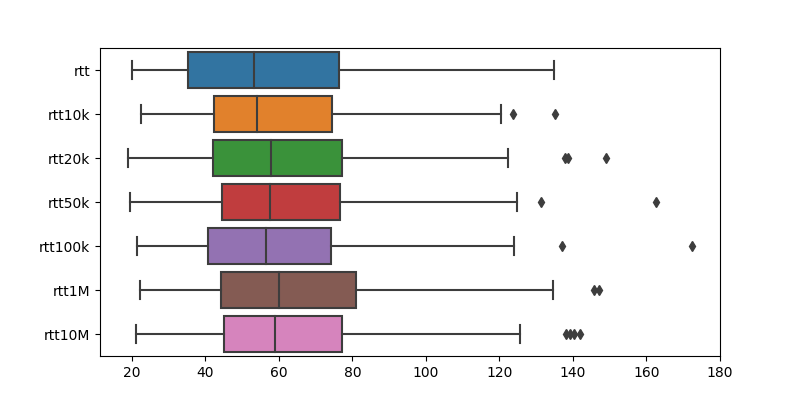
\includegraphics[width=1\textwidth]{pics/rtt-iperf-stress.png}
    \caption[short]{measuring RTT changes when applying stress iperf}
\end{figure}
\end{frame}

\begin{frame}{Visualize visible satellites}
\begin{itemize}
    \item from \href{celestrak.org}{celestrak.org} we can download a list of Starlink's satellites TLEs
    \item A two-line element set (TLE) is a data format encoding a list of orbital elements of an Earth-orbiting object for a given point in time, the epoch. Using a suitable prediction formula, the state (position and velocity) at any point in the past or future can be estimated to some accuracy. (from wikipedia.org)
\end{itemize}
\end{frame}

\begin{frame}[fragile]{\texttt{common.calculate\_visible\_satellites}}
\begin{minted}[fontsize=\small]{python3}
def calculate_visible_satellites(...):
    # ...
    satellites = load.tle_file(stations_url)
    observer = Topos(observer_latitude, observer_longitude, observer_elevation)
    t = load.timescale().now()

    # Calculate satellite positions
    positions = [(sat, (sat - observer).at(t)) for sat in satellites]
    
    # Filter visible satellites
    visible_satellites = []
    for sat, position in positions:
        alt, az, distance = position.altaz()
        # Satellite is above the horizon
        if alt.degrees > 0 and distance.km < distance_km:
            visible_satellites.append((sat, alt, az))

    return visible_satellites
\end{minted}
\end{frame}

\begin{frame}{count of visible satellites across time}
\begin{figure}
    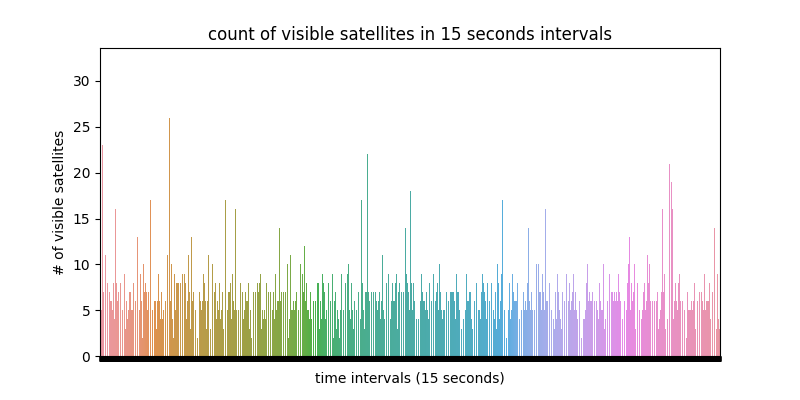
\includegraphics[width=1\textwidth]{pics/count_visible_satellites.png}
    \caption[short]{count of visible satellites across time}
\end{figure}
\end{frame}

\begin{frame}{visualizing patterns in visible satellites}
\begin{figure}
    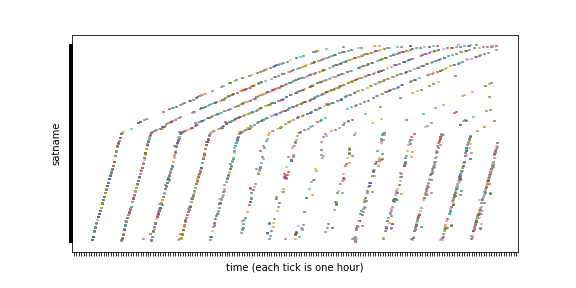
\includegraphics[width=1\textwidth]{pics/visualizing-how-long-satellites-are-visible-for.png}
    \caption[short]{visualizing patterns in visible satellites}
\end{figure}
\end{frame}

\begin{frame}{the gRPC api}
\begin{itemize}
    \item the dish exposes a gRPC api with server reflection, "runtime construction of requests without having stub information precompiled into the client." \footnote{\href{https://github.com/grpc/grpc/blob/master/doc/server-reflection.md}{https://github.com/grpc/grpc/blob/master/doc/server-reflection.md}}
    \item 55 "methods" are available, most of them don't work, we have 2 categories of errors: \texttt{Uninmplemented}, \texttt{PermissionDenied} and a couple of some other specific errors 
    \item working methods: \texttt{reboot}, \texttt{get\_status}, \texttt{start\_dish\_self\_test}, \texttt{get\_history}, \texttt{get\_device\_info}, \texttt{dish\_power\_save}, \texttt{dish\_get\_config}, \texttt{get\_obstruction\_map}
    \item to see all methods: \href{https://hedgedoc.net.in.tum.de/N7nACD1OSk2x2e7biPHJTA}{https://hedgedoc.net.in.tum.de/N7nACD1OSk2x2e7biPHJTA}
\end{itemize}
\end{frame}

\begin{frame}{next actions}
\begin{itemize}
    \item investigate satellite handovers following the method described in \cite{izhikevich2023democratizing} (we have a script working)
    \item try to correlate satellite handovers with sudden drops in bandwidth
    \item sneak peak: \href{https://youtu.be/PjfMPr20suw}{https://youtu.be/PjfMPr20suw}
\end{itemize}
\end{frame}

\section{Bibliography}
\begin{frame}[allowframebreaks]
    \bibliographystyle{abbrv}
    \setbeamertemplate{bibliography item}[text]
    \footnotesize
    \bibliography{lit}
\end{frame}

\end{document}


\begin{document}

\begin{frame}
    \begin{itemize}
        \item title for slides deck? should we change project's name?
        \item add bandwidth during downloads
        \item should I briefly explain how starlink works? figure 2 https://arxiv.org/pdf/2306.07469.pdf
        \item anything else to add?
    \end{itemize}
\end{frame}

\begin{frame}{Agenda}
    \begin{itemize}
        \item trying to understand routing decisions
        \item visualize visible satellites
        \item exploring the GRPC api
    \end{itemize}
\end{frame}
\begin{frame}{Understanding routing decisions}
    \begin{itemize}
        \item got ip address blocks from major cloud providers (aws,azure,oracle), as we know their position \footnote[]{the fact we know the position doesn't really mean a traceroute to a certain address is really a traceroute to that geographic area}
        \item chose 5 geographically sparse targets around the globe (for aws: ap-northeast-2, us-east-1, ap-south-1, sa-east-1, me-south-1 )
        \item tracerouted the targets over several days 
    \end{itemize}
\end{frame}

\begin{frame}{Understanding routing decisions}
    \begin{figure}
        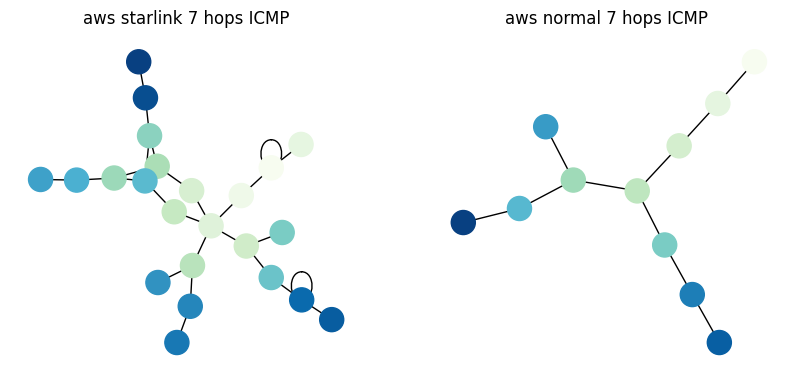
\includegraphics[width=0.75\textwidth]{pics/aws_7_icmp.png}
        \caption[short]{First 7 hops of traceroutes to 5 AWS datacenters using ICMP}
    \end{figure}
\end{frame}
\begin{frame}{Understanding routing decisions}
    \begin{figure}
        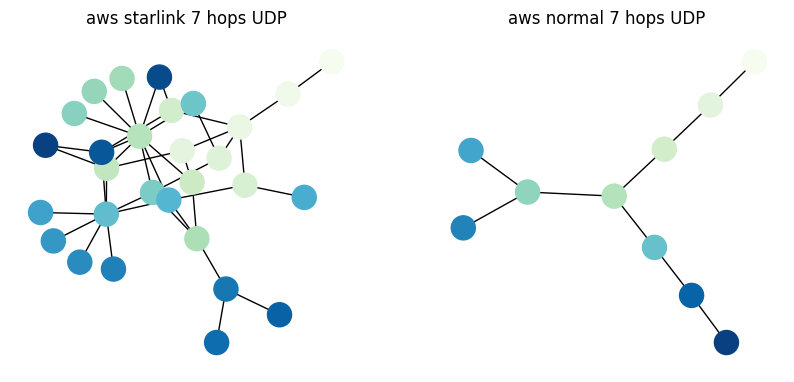
\includegraphics[width=0.75\textwidth]{pics/aws_7_udp.png}
        \caption[short]{First 7 hops of traceroutes to 5 AWS datacenters using UDP}
    \end{figure}
\end{frame}
\begin{frame}{Understanding routing decisions}
    \begin{figure}
        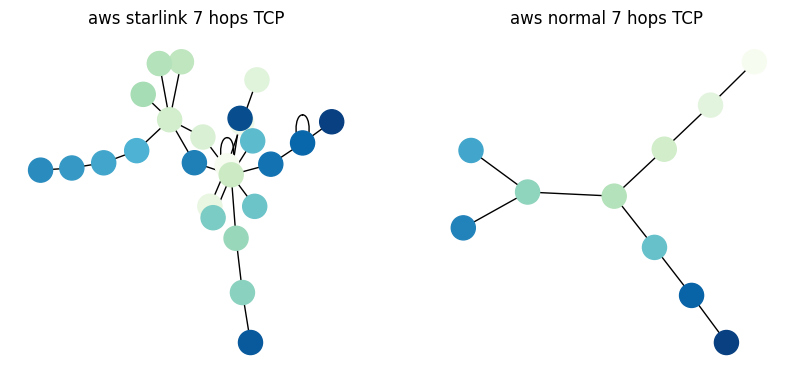
\includegraphics[width=0.75\textwidth]{pics/aws_7_tcp.png}
        \caption[short]{First 7 hops of traceroutes to 5 AWS datacenters using TCP}
    \end{figure}
\end{frame}

\begin{frame}{measuring RTT changes when applying stress iperf}
    \begin{figure}
        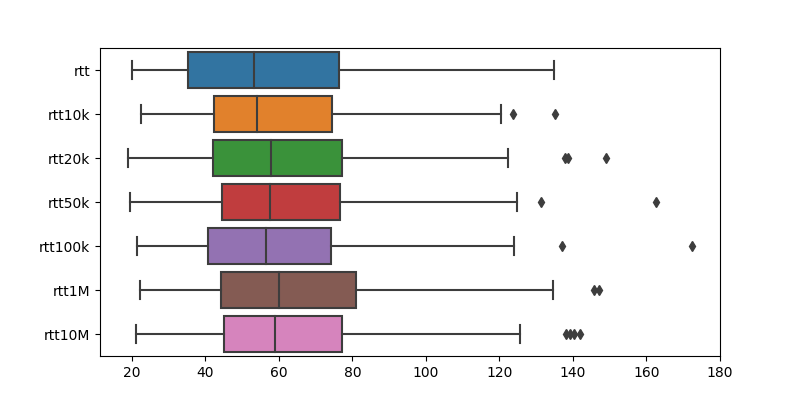
\includegraphics[width=1\textwidth]{pics/rtt-iperf-stress.png}
        \caption[short]{measuring RTT changes when applying stress iperf}
    \end{figure}
\end{frame}

\begin{frame}{Visualize visible satellites}
    \begin{itemize}
        \item from \href{celestrak.org}{celestrak.org} we can download a list of Starlink's satellites TLEs
        \item A two-line element set (TLE) is a data format encoding a list of orbital elements of an Earth-orbiting object for a given point in time, the epoch. Using a suitable prediction formula, the state (position and velocity) at any point in the past or future can be estimated to some accuracy. (from wikipedia.org)
    \end{itemize}
\end{frame}

\begin{frame}[fragile]{\texttt{common.calculate\_visible\_satellites}}
    \begin{minted}[fontsize=\small]{python3}
def calculate_visible_satellites(...):
    # ...
    satellites = load.tle_file(stations_url)
    observer = Topos(observer_latitude, observer_longitude, observer_elevation)
    t = load.timescale().now()

    # Calculate satellite positions
    positions = [(sat, (sat - observer).at(t)) for sat in satellites]
    
    # Filter visible satellites
    visible_satellites = []
    for sat, position in positions:
        alt, az, distance = position.altaz()
        # Satellite is above the horizon
        if alt.degrees > 0 and distance.km < distance_km:
            visible_satellites.append((sat, alt, az))

    return visible_satellites
    \end{minted}
\end{frame}

\begin{frame}{count of visible satellites across time}
    \begin{figure}
        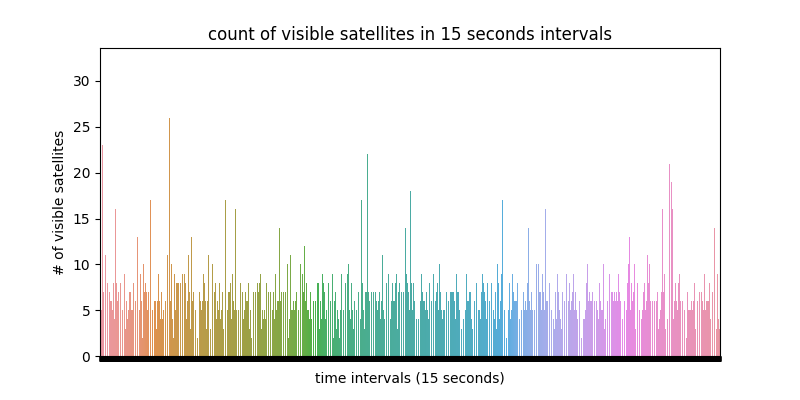
\includegraphics[width=1\textwidth]{pics/count_visible_satellites.png}
        \caption[short]{count of visible satellites across time}
    \end{figure}
\end{frame}

\begin{frame}{visualizing patterns in visible satellites}
    \begin{figure}
        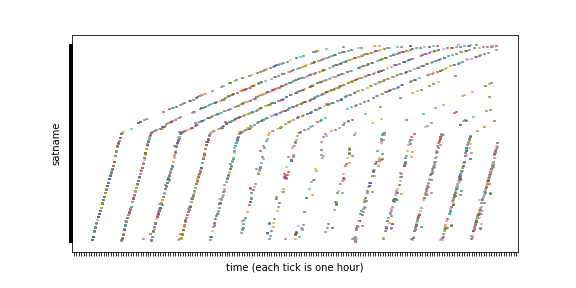
\includegraphics[width=1\textwidth]{pics/visualizing-how-long-satellites-are-visible-for.png}
        \caption[short]{visualizing patterns in visible satellites}
    \end{figure}
\end{frame}

\begin{frame}{the gRPC api}
    \begin{itemize}
        \item the dish exposes a gRPC api with server reflection, "runtime construction of requests without having stub information precompiled into the client." \footnote{\href{https://github.com/grpc/grpc/blob/master/doc/server-reflection.md}{https://github.com/grpc/grpc/blob/master/doc/server-reflection.md}}
        \item 55 "methods" are available, most of them don't work, we have 2 categories of errors: \texttt{Uninmplemented}, \texttt{PermissionDenied} and a couple of some other specific errors 
        \item working methods: \texttt{reboot}, \texttt{get\_status}, \texttt{start\_dish\_self\_test}, \texttt{get\_history}, \texttt{get\_device\_info}, \texttt{dish\_power\_save}, \texttt{dish\_get\_config}, \texttt{get\_obstruction\_map}
        \item to see all methods: \href{https://hedgedoc.net.in.tum.de/N7nACD1OSk2x2e7biPHJTA}{https://hedgedoc.net.in.tum.de/N7nACD1OSk2x2e7biPHJTA}
    \end{itemize}
\end{frame}

% \section{Bibliography}
% \begin{frame}[allowframebreaks]
%     \bibliographystyle{abbrv}
%     \setbeamertemplate{bibliography item}[text]
%     \footnotesize
%     \bibliography{lit}
% \end{frame}



\end{document}
